% Class final report using the Interspeech 2026 Paper Kit format:
% https://www.overleaf.com/latex/templates/interspeech-paper-kit/svqkgcpdbxfg

\documentclass[cameraready]{Interspeech}

\title{Read or Spontaneous? Speech Style Effects on Speaker Verification for L2 English}

\author[affiliation={1}]{Lina}{Na}
\address{$^1$ University of Zurich, Switzerland}
\email{lina.na@uzh.ch}

\keywords{speaker verification, L2 English, speaking style}

\usepackage{booktabs,multirow,tikz}

\begin{document}
\maketitle

\begin{abstract}
Automatic speaker verification (ASV) systems authenticate individuals from short speech segments, and are increasingly deployed in voice-based access control, mobile banking, and language-learning applications. Most benchmark evaluations nevertheless assume that enrollment and test utterances share the same speaking style. Read or scripted speech is typically fluent and acoustically stable, whereas spontaneous speech contains hesitations, restarts, and variable articulation that change short-term spectral structure. Prior work on native English shows that such style mismatch raises equal error rate (EER), but comparatively little evidence exists for non-native (L2) talkers, whose pronunciation varies with first-language (L1) transfer. This study evaluates two widely used embedding extractors---TDNN x-vector and ECAPA-TDNN, both pretrained on VoxCeleb and distributed via SpeechBrain---on two publicly available L2 English corpora: L2-ARCTIC (24 speakers, six L1 backgrounds, read and spontaneous suitcase speech) and Svarah (117 Indian-accented speakers, read and conversational material). For each corpus and model we construct speaker verification trials under three conditions: Read--Read (matched), Spontaneous--Spontaneous (matched), and Read--Spontaneous (enroll read, test spontaneous, mismatched). Performance is measured by EER without model fine-tuning. On Svarah, both models follow the expected trend: Read--Read yields the lowest EER (x-vector: 6.09\%; ECAPA: 2.09\%), Spontaneous--Spontaneous is substantially harder (28.53\% and 12.57\%), and Read--Spontaneous remains degraded (25.09\% and 10.55\%). ECAPA-TDNN is consistently more robust than x-vector. L2-ARCTIC results are less conclusive because spontaneous material is sparse (22 speakers, one long recording each, segmented into approximately 10\,s chunks); nevertheless, Read--Spontaneous mismatch increases x-vector EER from 6.25\% to 8.18\%. Code, data-processing scripts, and evaluation results are available at \url{https://github.com/NeoCitran-oss/myFinal}.
\end{abstract}

\section{Introduction}
\label{sec:intro}

Speaker verification (SV) is the task of deciding whether two speech segments were produced by the same person. Modern text-independent systems map each utterance to a fixed-dimensional embedding using a neural network, then compare embeddings with cosine similarity~\cite{snyder2018xvector,desplanques2020ecapa}. When enrollment and test speech are drawn from similar acoustic conditions, pretrained models such as x-vector and ECAPA-TDNN achieve strong performance on benchmarks built from celebrity interviews and read prompts~\cite{chung2018voxceleb,desplanques2020ecapa}.

Real deployments rarely preserve those conditions. A user may enroll with a prompted passphrase or read sentence, but authenticate while speaking freely during a customer-service call or a language-practice session. Read speech is more controlled: speakers follow a script, maintain steadier rate, and produce fewer disfluencies. Spontaneous speech introduces pauses, filled pauses, lexical searches, and prosodic variation that alter frame-level acoustics even when the talker's identity is unchanged~\cite{kenny2014style}. Several studies report that enrollment--test \emph{speaking-style mismatch} increases verification error on native English material~\cite{tom2010style,afshan2015style,wang2020crossstyle}. The problem is plausibly stronger for L2 English speakers, whose phones and rhythm reflect L1 transfer and who may read more carefully than they speak spontaneously~\cite{zhao2018l2arctic}.

Despite India's position as one of the largest English-using populations worldwide, Indian-accented talkers remain underrepresented in standard verification benchmarks~\cite{javed2023svarah}. L2-ARCTIC fills part of this gap with non-native read English from multiple L1 backgrounds and a smaller spontaneous subset~\cite{zhao2018l2arctic}. Svarah provides read and conversational Indian-accented English designed for ASR evaluation~\cite{javed2023svarah}. Neither corpus has been studied extensively for multi-style speaker verification with modern embedding models.

This report addresses the following research question: \emph{How does speaking style (read vs.\ spontaneous/conversational) affect off-the-shelf x-vector and ECAPA-TDNN verification on L2 English?} We do not propose a new architecture; instead we quantify a deployment-relevant failure mode using reproducible trials and publicly available checkpoints~\cite{ravanelli2021speechbrain}. Our contributions are: (i) a unified evaluation protocol with three style conditions on two L2 corpora; (ii) empirical EER comparisons between x-vector and ECAPA-TDNN; and (iii) an open-source pipeline for downloading data, building indices, and reporting results (\url{https://github.com/NeoCitran-oss/myFinal}).

\section{Related work}
\label{sec:related}

\subsection{Speaker embedding models}

The x-vector architecture stacks time-delay neural network (TDNN) layers with statistics pooling to produce utterance-level embeddings~\cite{snyder2018xvector}. Training on large-scale speaker-labeled data (e.g., VoxCeleb) with a classification loss yields embeddings that generalize to unseen speakers via cosine scoring. ECAPA-TDNN extends this design with attentive statistics pooling, channel attention, and multi-layer feature aggregation~\cite{desplanques2020ecapa}. On many verification benchmarks ECAPA achieves lower EER than classical x-vector systems, especially under noise and channel variability~\cite{desplanques2020ecapa}. SpeechBrain distributes pretrained VoxCeleb models for both architectures, enabling consistent off-the-shelf evaluation~\cite{ravanelli2021speechbrain,chung2018voxceleb}. Figure~\ref{fig:sota} contrasts the two pipelines used in our experiments.

\begin{figure}[t]
  \centering
  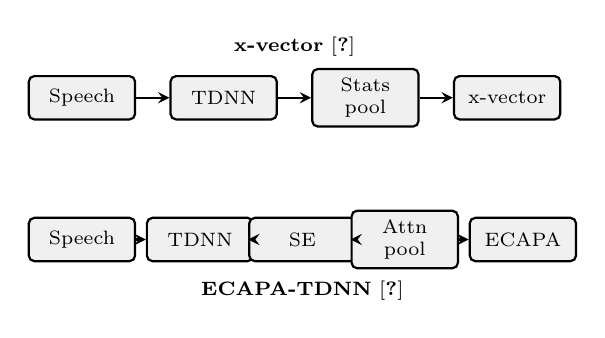
\begin{tikzpicture}[font=\scriptsize, >=stealth, thick]
    \tikzstyle{block}=[draw, rounded corners=2pt, minimum height=0.55cm, minimum width=1.35cm, align=center, fill=gray!12]
    \node[block] (in1) at (0,0.9) {Speech};
    \node[block] (tdnn1) at (1.8,0.9) {TDNN};
    \node[block] (pool1) at (3.6,0.9) {Stats\\pool};
    \node[block] (out1) at (5.4,0.9) {x-vector};
    \draw[->] (in1) -- (tdnn1); \draw[->] (tdnn1) -- (pool1); \draw[->] (pool1) -- (out1);
    \node at (2.7,1.55) {\textbf{x-vector}~\cite{snyder2018xvector}};
    \node[block] (in2) at (0,-0.9) {Speech};
    \node[block] (tdnn2) at (1.5,-0.9) {TDNN};
    \node[block] (se) at (2.8,-0.9) {SE};
    \node[block] (apool) at (4.1,-0.9) {Attn\\pool};
    \node[block] (out2) at (5.6,-0.9) {ECAPA};
    \draw[->] (in2) -- (tdnn2); \draw[->] (tdnn2) -- (se);
    \draw[->] (se) -- (apool); \draw[->] (apool) -- (out2);
    \node at (2.8,-1.55) {\textbf{ECAPA-TDNN}~\cite{desplanques2020ecapa}};
  \end{tikzpicture}
  \caption{State-of-the-art speaker embedding pipelines evaluated in this study. x-vector uses frame-level TDNN features with statistics pooling; ECAPA-TDNN adds squeeze--excitation (SE) channel attention and attentive statistics pooling for more robust embeddings.}
  \label{fig:sota}
\end{figure}

\subsection{Speaking style and verification}

Speaker recognition research has long noted sensitivity to train--test condition mismatch. Kenny \textit{et al.}~\cite{kenny2014style} discussed verification with short segments under mismatched conditions in NIST-style evaluations. Tom \textit{et al.}~\cite{tom2010style} examined read versus conversational speech in forensic-style settings. Afshan \textit{et al.}~\cite{afshan2015style} showed that regional and stylistic variability negatively affects automatic speaker comparison in forensic casework. More recent embedding-based systems inherit this sensitivity: models trained predominantly on read or interview speech can underperform when test segments are conversational~\cite{wang2020crossstyle}. These findings motivate explicit reporting of enrollment and test style in verification experiments.

\subsection{L2 and accented English corpora}

L2-ARCTIC~\cite{zhao2018l2arctic} contains read English from 24 non-native speakers spanning Arabic, Hindi, Korean, Mandarin, Spanish, and Vietnamese L1 backgrounds, plus manual pronunciation annotations on a subset. The suitcase corpus adds spontaneous picture-description speech from 22 speakers. Svarah~\cite{javed2023svarah} comprises 9.6 hours of transcribed Indian-accented English from 117 speakers across 19 states, with both read passages and conversational prompts (e.g., government services, digital payments). While both corpora are widely used in ASR and pronunciation research, systematic speaker-verification trials across matched and mismatched speaking styles on L2 talkers remain limited.

\section{Limitations of current practice}
\label{sec:pitfalls}

Three limitations of common verification practice motivate our study.

\textbf{Benchmark bias.} Pretrained x-vector and ECAPA models are optimized on VoxCeleb interview and read-like speech from mostly native talkers~\cite{chung2018voxceleb,desplanques2020ecapa}. L2 English with accent variability and spontaneous disfluencies constitutes an out-of-domain test. Reporting VoxCeleb EER alone therefore overestimates readiness for L2 deployment.

\textbf{Hidden protocol mismatch.} Papers often report a single corpus-level EER without stating enrollment and test speaking style. A system evaluated only on read--read trials may appear production-ready while failing when users authenticate spontaneously~\cite{tom2010style}. Explicit style-conditioned protocols are necessary for interpretable conclusions.

\textbf{Sparse spontaneous coverage.} Matched spontaneous--spontaneous trials require at least two spontaneous segments per speaker. Corpora with one long spontaneous recording per talker---as in L2-ARCTIC suitcase data---force chunking or exclusion of speakers, weakening SS evaluation~\cite{zhao2018l2arctic}. Corpus design directly affects which conclusions can be drawn about spontaneous verification.

\section{Proposed evaluation framework}
\label{sec:method}

\subsection{Verification protocol}

We adopt standard text-independent speaker verification. For each target speaker, one utterance from the enrollment style is used to compute an embedding $\bar{e}$ (mean over enrollment segments; here a single segment). A test utterance from the test style yields embedding $e_t$. The score is cosine similarity $\cos(\bar{e}, e_t)$. A target trial uses the same speaker for enrollment and test; impostor trials pair the test utterance with enrollment embeddings from different speakers, using the same enrollment style as the target trial.

Equal error rate (EER) is the threshold at which false acceptance rate equals false rejection rate~\cite{snyder2018xvector}. We sweep thresholds over all trial scores per condition and report EER in percent.

\subsection{Style conditions}

Three conditions are evaluated for each corpus and model:
\begin{itemize}
  \item \textbf{Read--Read (RR):} enrollment and test on read/scripted speech (matched).
  \item \textbf{Spontaneous--Spontaneous (SS):} enrollment and test on spontaneous or conversational speech (matched).
  \item \textbf{Read--Spontaneous (RS):} enrollment on read speech, test on spontaneous speech (mismatched).
\end{itemize}

Based on prior native-speaker studies~\cite{tom2010style,wang2020crossstyle}, we expect RS (and often SS) to yield higher EER than RR, with ECAPA more robust than x-vector~\cite{desplanques2020ecapa}.

\subsection{Models and scoring}

We use SpeechBrain checkpoints \texttt{spkrec-xvect-voxceleb} and \texttt{spkrec-ecapa-voxceleb}~\cite{ravanelli2021speechbrain} without fine-tuning. Audio is converted to mono and resampled to \SI{16}{\kilo\hertz}. No score normalization or cohort-based calibration is applied, isolating raw embedding behavior on L2 data.

Figure~\ref{fig:protocol} illustrates the trial flow. Table~\ref{tab:protocol} lists hyperparameters. Table~\ref{tab:trialcounts} reports trial counts per condition.

\begin{figure}[t]
  \centering
  \fbox{\parbox{0.92\linewidth}{\centering\vspace{0.8em}
  \small
  \textbf{Step 1:} Select enrollment utterance(s) in style A \\
  $\rightarrow$ extract embedding(s) $\rightarrow$ $\bar{e}$ \\
  \textbf{Step 2:} Select test utterance in style B $\rightarrow$ $e_t$ \\
  \textbf{Step 3:} score $= \cos(\bar{e}, e_t)$ \\
  Target trial: same speaker; impostor trial: different speaker \\
  \vspace{0.8em}}}
  \caption{Speaker verification trial construction for enrollment style A and test style B. RR uses A=B=read; SS uses A=B=spontaneous; RS enrolls read and tests spontaneous speech.}
  \label{fig:protocol}
\end{figure}

\begin{table}[t]
  \caption{Shared experimental settings for all datasets and models. Each target trial is paired with five impostor trials drawn from other speakers using the same enrollment style.}
  \label{tab:protocol}
  \centering
  \begin{tabular}{ll}
    \toprule
    Setting & Value \\
    \midrule
    Sample rate & \SI{16}{\kilo\hertz} \\
    Enrollment utterances & 1 \\
    Impostors per target trial & 5 \\
    Scoring & Cosine similarity \\
    Metric & Equal error rate (EER) \\
    Random seed & 42 \\
    \bottomrule
  \end{tabular}
\end{table}

\section{Datasets}
\label{sec:datasets}

\subsection{L2-ARCTIC}

L2-ARCTIC~\cite{zhao2018l2arctic} includes read sentences from 24 non-native English speakers (four talkers per L1: Arabic, Hindi, Korean, Mandarin, Spanish, Vietnamese). The suitcase spontaneous corpus contains picture descriptions from 22 of the 24 speakers~\cite{zhao2018l2arctic}. We use the KoelLabs HuggingFace release~\cite{koellabs2024l2arctic}: 3{,}599 scripted utterances and 22 spontaneous source recordings.

Because each speaker contributes only one long spontaneous recording, matched SS trials require multiple segments per speaker. We split each spontaneous waveform into approximately \SI{10}{\second} chunks, yielding 162 spontaneous segments ($\sim$7.4 per speaker on average). This follows the spirit of published spontaneous splits for the same corpus, but remains a limitation: chunks from one session are acoustically correlated.

\subsection{Svarah}

Svarah~\cite{javed2023svarah} contains 9.6 hours of Indian-accented English from 117 speakers across 65 districts and 19 states. Material includes read passages (history, culture, tourism) and conversational prompts (e.g., passport status, scholarship applications, grocery ordering). The public HuggingFace \texttt{test} split does not ship an explicit read/conversational label. We infer style from transcript text: interrogatives, service-oriented vocabulary, and short replies are labeled spontaneous; narrative read passages are labeled read. After filtering, 110 speaker profiles contain both inferred styles. This heuristic should be replaced with official metadata if released.

\subsection{Data acquisition}

Both corpora are downloaded with our \texttt{download.py} script (HuggingFace \texttt{datasets} API, \texttt{hf auth login} required for gated releases). Waveforms and JSON indices are stored locally; see the repository README at \url{https://github.com/NeoCitran-oss/myFinal} for setup instructions (\texttt{setup\_env.sh}, conda environment \texttt{l2-spkverif}).

\section{Hypotheses}
\label{sec:hypotheses}

Based on prior work on style mismatch~\cite{tom2010style,wang2020crossstyle} and ECAPA robustness~\cite{desplanques2020ecapa}, we test three hypotheses:
\begin{itemize}
  \item \textbf{H1 (style mismatch):} Read--Spontaneous and Spontaneous--Spontaneous trials yield higher EER than Read--Read trials on L2 corpora.
  \item \textbf{H2 (model robustness):} ECAPA-TDNN yields lower EER than x-vector across all style conditions.
  \item \textbf{H3 (corpus effect):} Style effects are stronger on Svarah than on L2-ARCTIC because Svarah provides more spontaneous material per speaker.
\end{itemize}

\section{Experiments}
\label{sec:experiments}

\subsection{Implementation}

The evaluation pipeline consists of four components, all available on GitHub (\url{https://github.com/NeoCitran-oss/myFinal}):
\begin{itemize}
  \item \texttt{config.py} --- paths, model IDs, trial settings;
  \item \texttt{core.py} --- index I/O, trial generation, embedding extraction, EER;
  \item \texttt{download.py} --- dataset download and index building;
  \item \texttt{run\_eval.py} --- end-to-end evaluation and \texttt{summary.json} output;
  \item \texttt{run\_ablation\_enroll.py} --- enrollment-length ablation on Svarah RR.
\end{itemize}

Indices map each waveform to speaker ID, style (read or spontaneous), and file path. Trials are generated programmatically for all three conditions with fixed random seed 42. Embeddings are extracted with SpeechBrain \texttt{EncoderClassifier.encode\_batch}; enrollment embeddings average over the selected enrollment file(s). EER is computed per dataset, model, and condition.

\subsection{Compute environment}

Experiments were run on a Linux server (\texttt{--device auto}; CUDA was unavailable during ablation, so those runs used CPU). Model weights are cached under \texttt{hf\_cache/}. No hyperparameter search was performed on the main experiments; we report off-the-shelf checkpoint behavior only.

\subsection{Ablation: enrollment length}

We ablate the number of enrollment utterances on Svarah Read--Read trials, comparing one vs.\ two read enrollment segments (test protocol unchanged). Averaging two enrollment embeddings should stabilize speaker estimates and may lower EER~\cite{snyder2018xvector}. Results are reported in Table~\ref{tab:ablation}.

\subsection{Speaker coverage}

Table~\ref{tab:trialcounts} summarizes speakers and trials. L2-ARCTIC RR includes all 24 read speakers; SS and RS include 22 speakers with spontaneous material. Svarah RR and RS use 110 speakers; SS uses 109 speakers with at least two spontaneous segments.

\begin{table}[t]
  \caption{Number of target speakers and total verification trials (target + impostor) per corpus and condition for the x-vector system (trial counts are identical across models).}
  \label{tab:trialcounts}
  \centering
  \begin{tabular}{lcccc}
    \toprule
    Corpus & Condition & Target spk. & Trials \\
    \midrule
    \multirow{3}{*}{L2-ARCTIC} & RR & 24 & 144 \\
     & SS & 22 & 132 \\
     & RS & 22 & 132 \\
    \midrule
    \multirow{3}{*}{Svarah} & RR & 110 & 660 \\
     & SS & 109 & 654 \\
     & RS & 110 & 660 \\
    \bottomrule
  \end{tabular}
\end{table}

\section{Results}
\label{sec:results}

Table~\ref{tab:results} reports EER (\%) for all corpus--model--condition combinations. Figure~\ref{fig:eer_compare} summarizes the Svarah trend, where style effects are most pronounced.

\subsection{Svarah}

On Svarah, results align with the hypothesis from native-speaker style-mismatch work~\cite{tom2010style,wang2020crossstyle}. \textbf{Read--Read} achieves the lowest EER for both models (x-vector: 6.09\%; ECAPA: 2.09\%). \textbf{Spontaneous--Spontaneous} is substantially harder (28.53\% and 12.57\%), reflecting conversational variability, short replies, and domain-specific vocabulary in service-oriented prompts~\cite{javed2023svarah}. \textbf{Read--Spontaneous} mismatch remains high (25.09\% and 10.55\%), confirming that enrolling with read speech does not reliably authenticate spontaneous test segments.

ECAPA-TDNN outperforms x-vector in every condition, consistent with its stronger channel and noise modeling~\cite{desplanques2020ecapa}. The absolute gap is largest under SS (16 percentage points), suggesting ECAPA's attentive pooling helps under spontaneous variability. For deployment on Indian-accented L2 English, ECAPA is preferable among these two off-the-shelf choices, but RS EER above 10\% still indicates practical risk without adaptation.

\subsection{L2-ARCTIC}

L2-ARCTIC tells a more nuanced story. ECAPA achieves near-zero EER across conditions (0.00--0.45\%), likely because the studio-quality read corpus is small and relatively easy for a strong VoxCeleb-trained model. x-vector shows higher absolute EER. \textbf{Read--Spontaneous} (8.18\%) exceeds \textbf{Read--Read} (6.25\%), supporting the mismatch hypothesis on this subset. Unexpectedly, \textbf{Spontaneous--Spontaneous} (2.27\%) is \emph{lower} than RR for x-vector---probably an artifact of (i) only 22 speakers, (ii) correlated 10\,s chunks from single suitcase sessions, and (iii) different trial pool sizes, rather than genuine spontaneous robustness.

\subsection{Cross-corpus comparison}

Svarah exhibits clearer style effects than L2-ARCTIC, likely because it offers more spontaneous material per speaker and broader conversational coverage. L2-ARCTIC remains valuable for multi-L1 read speech but is a weak standalone corpus for spontaneous verification without additional sessions or official spontaneous splits~\cite{zhao2018l2arctic}. Both corpora together illustrate that \emph{corpus design and trial construction} shape scientific conclusions as much as model choice.

\subsection{Hypothesis summary}

\textbf{H1} is supported on Svarah (RR $<$ RS $\approx$ SS) but only partially on L2-ARCTIC (RS $>$ RR for x-vector; SS unexpectedly low). \textbf{H2} is supported on both corpora: ECAPA-TDNN consistently outperforms x-vector. \textbf{H3} is supported: Svarah shows larger EER spreads across conditions than L2-ARCTIC.

\subsection{Ablation results}

Table~\ref{tab:ablation} shows that using two enrollment utterances improves Svarah RR performance for both models (x-vector: 6.09\% $\rightarrow$ 3.85\%; ECAPA: 2.09\% $\rightarrow$ 1.38\%), confirming that enrollment length affects EER even under matched read--read conditions.

\begin{table}[t]
  \caption{Ablation on Svarah Read--Read: EER (\%) vs.\ number of enrollment utterances.}
  \label{tab:ablation}
  \centering
  \begin{tabular}{lcc}
    \toprule
    Model & 1 enroll utt. & 2 enroll utts. \\
    \midrule
    x-vector & 6.09 & 3.85 \\
    ECAPA-TDNN & 2.09 & 1.38 \\
    \bottomrule
  \end{tabular}
\end{table}

\begin{table}[t]
  \caption{Equal error rate (EER, \%) on L2-ARCTIC and Svarah for x-vector and ECAPA-TDNN under three enrollment--test style conditions. RR: read--read; SS: spontaneous--spontaneous; RS: read enrollment with spontaneous test. L2-ARCTIC spontaneous trials use $\sim$\SI{10}{\second} chunks from single suitcase recordings per speaker.}
  \label{tab:results}
  \centering
  \begin{tabular}{llccc}
    \toprule
    Corpus & Model & RR & SS & RS \\
    \midrule
    \multirow{2}{*}{L2-ARCTIC} & x-vector & 6.25 & 2.27 & 8.18 \\
     & ECAPA-TDNN & 0.00 & 0.45 & 0.00 \\
    \midrule
    \multirow{2}{*}{Svarah} & x-vector & 6.09 & 28.53 & 25.09 \\
     & ECAPA-TDNN & 2.09 & 12.57 & 10.55 \\
    \bottomrule
  \end{tabular}
\end{table}

\begin{figure}[t]
  \centering
  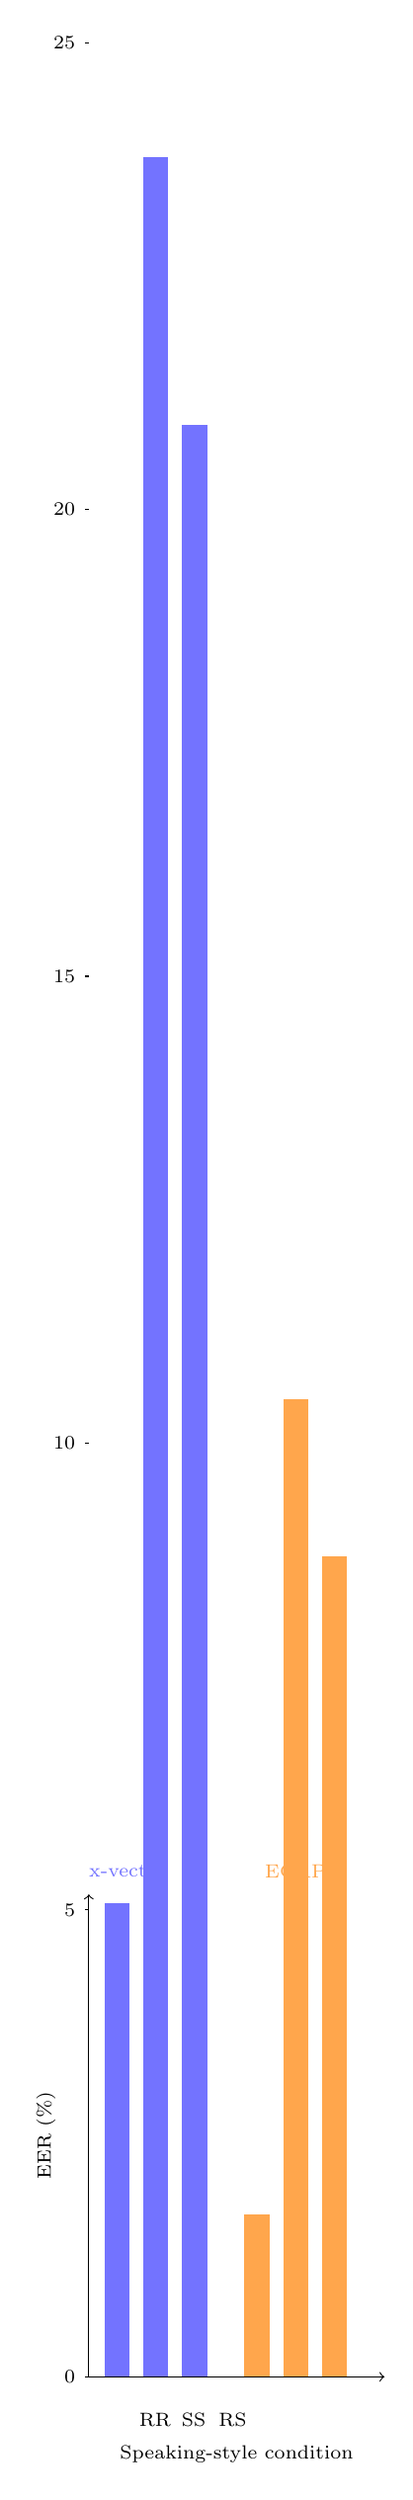
\begin{tikzpicture}[font=\scriptsize]
    \def\barwidth{0.32}
    \def\ymax{30}
    % x-vector bars
    \fill[blue!55] (0.2,0) rectangle (0.2+\barwidth,6.09/30*\ymax);
    \fill[blue!55] (0.7,0) rectangle (0.7+\barwidth,28.53/30*\ymax);
    \fill[blue!55] (1.2,0) rectangle (1.2+\barwidth,25.09/30*\ymax);
    % ECAPA bars
    \fill[orange!70] (2.0,0) rectangle (2.0+\barwidth,2.09/30*\ymax);
    \fill[orange!70] (2.5,0) rectangle (2.5+\barwidth,12.57/30*\ymax);
    \fill[orange!70] (3.0,0) rectangle (3.0+\barwidth,10.55/30*\ymax);
    % axes
    \draw[->] (0,0) -- (3.8,0);
    \draw[->] (0,0) -- (0,\ymax/30*6.2);
    \foreach \y/\lbl in {0/0, 6/5, 12/10, 18/15, 24/20, 30/25} {
      \draw (0,\y/30*\ymax) -- (-0.05,\y/30*\ymax) node[left] {\lbl};
    }
    \node at (0.85,-0.55) {RR};
    \node at (1.35,-0.55) {SS};
    \node at (1.85,-0.55) {RS};
    \node[blue!55] at (0.5,6.5) {x-vector};
    \node[orange!70] at (2.75,6.5) {ECAPA};
    \node at (1.9,-1.0) {Speaking-style condition};
    \node[rotate=90] at (-0.55,3.1) {EER (\%)};
  \end{tikzpicture}
  \caption{Svarah EER (\%) by speaking-style condition and model. Read--Read (RR) achieves the lowest error; Spontaneous--Spontaneous (SS) and Read--Spontaneous (RS) show substantial degradation, especially for x-vector.}
  \label{fig:eer_compare}
\end{figure}

\section{Conclusions and future work}
\label{sec:conclusion}

This study quantified how speaking style affects off-the-shelf x-vector and ECAPA-TDNN speaker verification on L2 English. Using a reproducible three-condition protocol on L2-ARCTIC and Svarah, we found that Svarah clearly exhibits the expected pattern: matched read verification is easiest, spontaneous and read--spontaneous conditions are substantially harder, and ECAPA-TDNN is more robust than x-vector~\cite{desplanques2020ecapa}. L2-ARCTIC partially supports read--spontaneous mismatch effects for x-vector but is limited by sparse spontaneous data and near-ceiling ECAPA performance.

These results matter for practical systems that enroll L2 users with scripted prompts but authenticate on free speech---for example language-learning apps or voice biometrics in multilingual markets~\cite{javed2023svarah,zhao2018l2arctic}. Reporting only read--read EER would overstate system readiness.

Future work should: (i) incorporate corpora with multiple independent spontaneous sessions per speaker; (ii) fine-tune or adapt embeddings on multi-style L2 data; (iii) replace heuristic Svarah style labels with official metadata; (iv) add score normalization and calibration; and (v) stratify results by L1 background across the six L2-ARCTIC language groups. Code and instructions for reproducing all experiments are available at \url{https://github.com/NeoCitran-oss/myFinal}.

\section{Acknowledgments}
This report was prepared as a final project at the University of Zurich using the Interspeech paper format. The author thanks course instructors and teaching assistants for feedback. Implementation code and results are hosted at \url{https://github.com/NeoCitran-oss/myFinal}.

\section{Generative AI Use Disclosure}
Generative AI tools were used for code development, manuscript editing, and LaTeX formatting assistance. The author reviewed all content and takes full responsibility for the report.

\bibliographystyle{IEEEtran}
\bibliography{references}

\end{document}
